% !TeX spellcheck = en_EN-English
\documentclass[a4paper]{article}
\usepackage[slovak]{babel}
\usepackage[utf8]{inputenc}
\usepackage[T1]{fontenc}
\usepackage{a4wide}
\usepackage{amsmath}
\usepackage{amsfonts}
\usepackage{amssymb}
\usepackage{mathrsfs}
\usepackage[small,bf]{caption}
\usepackage{subcaption}
\usepackage{xcolor}
\usepackage{graphicx}
\usepackage{enumerate}
\usepackage{hyperref}



\pagestyle{empty}
\setlength{\parindent}{0pt}

\newenvironment{modenumerate}
{\enumerate\setupmodenumerate}
{\endenumerate}

\newif\ifmoditem
\newcommand{\setupmodenumerate}{%
	\global\moditemfalse
	\let\origmakelabel\makelabel
	\def\moditem##1{\global\moditemtrue\def\mesymbol{##1}\item}%
	\def\makelabel##1{%
		\origmakelabel{##1\ifmoditem\rlap{\mesymbol}\fi\enspace}%
		\global\moditemfalse}%
}

\renewcommand{\thesubsection}{\alph{subsection})}

\makeatletter
\def\@seccntformat#1{%
	\expandafter\ifx\csname c@#1\endcsname\c@section\else
	\csname the#1\endcsname\quad
	\fi}
\makeatother

\begin{document} 
	
	\pagenumbering{arabic}
	\pagestyle{plain}
	
	\begin{center}
		\sc\large
		MBI Homework 3 for CS students
	\end{center}
	
	Autor: Marián Kravec
	\section{1. RNA structure and dynamic programming.}
	
	\subsection{}
	
	%\centerline{\includegraphics[width=0.7\textwidth]{podorysy}} 
	
	To compute structure with maximal number of base pairs without any not nested cases we will use slightly modified Nussinov algorithm.
	
	\centerline{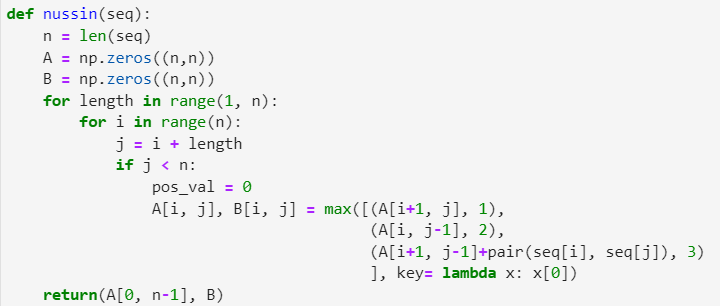
\includegraphics[width=0.7\textwidth]{nussin_1}}
	
	This algorithm is filling out table $A$ (starting from diagonal and getting closer to upper-top corner) where $A[i, j]$ is number maximal number of nested base pair of sub-sequence starting from position $i$ and ending on position $j$ (final solution is in cell $A[0, n]$ where $n$ is length of sequence), it's a bit simple than standard Nussinov algorithm because it does not take into account situation where branching of secondary structure create more base pairs, so situation where we are looking for position $k$ between positions $i$ and  $j$ such that $A[i, k]+A[k+1, j]$ is bigger than any other solution. We omit this rules because breaching creates not nested pairs.
	\\
	\\
	So to compute $A[i, j]$ our algorithm choose maximal value out of three possibilities: $A[i+1, j]$, $A[i, j-1]$ or $A[i+1, j-1]+pair(x_i, x_j)$. 
	\begin{itemize}
		\item{$A[i+1, j]$} - first base of sub-sequence in unpaired and rest is optimally paired 
		\item{$A[i+1, j]$} - last base of sub-sequence in unpaired and rest is optimally paired 
		\item{$A[i+1, j-1]+pair(x_i, x_j)$} - interpretation of this depends on value of $pair(x_i, x_j)$ if $x_i$ and $x_j$ creates pair then this is situation where we take optimal pairing of bases between them plus their own, if they do not create pair then this is situation where we take optimal pairing ob bases between them and first and last base is unpaired
	\end{itemize}
	
	% ADD SOMETHING ABOUT INTERPRETETATION OF STRUCTURE AS LIST OF BASE PAIR
	
	This algorithm compute half of values of matrix with size $n \times n$ and for each position if finds maximum of constant amount of possibilities (only 3), so asymptotic running time of this algorithm is $O(n^2)$.
	
	\subsection{}
	
	Similarly to algorithm from part a), our stochastic context-free grammar needs only one nonterminal which we will call $S$ and to have only three types of rules (three types does not mean three rules), and that is rules to create unpaired bases before nonterminal, rules to create unpaired bases after nonterminal and rules to create pairs (and lastly there will be rule to terminate sequence generation):
	
	\begin{align*}
		S \rightarrow & aS | uS | cS | gS |
		\\
		&Sa | Su | Sc | Sg | 
		\\
		&aSu | uSa | cSg | gSc | 
		\\
		&\epsilon 
	\end{align*}

	\subsection{}
	%TODO
	
	\section{2. Bioinformatics tools and databases.}
	
	\subsection{}
	
	After running Blast with in this setup:
	
	\centerline{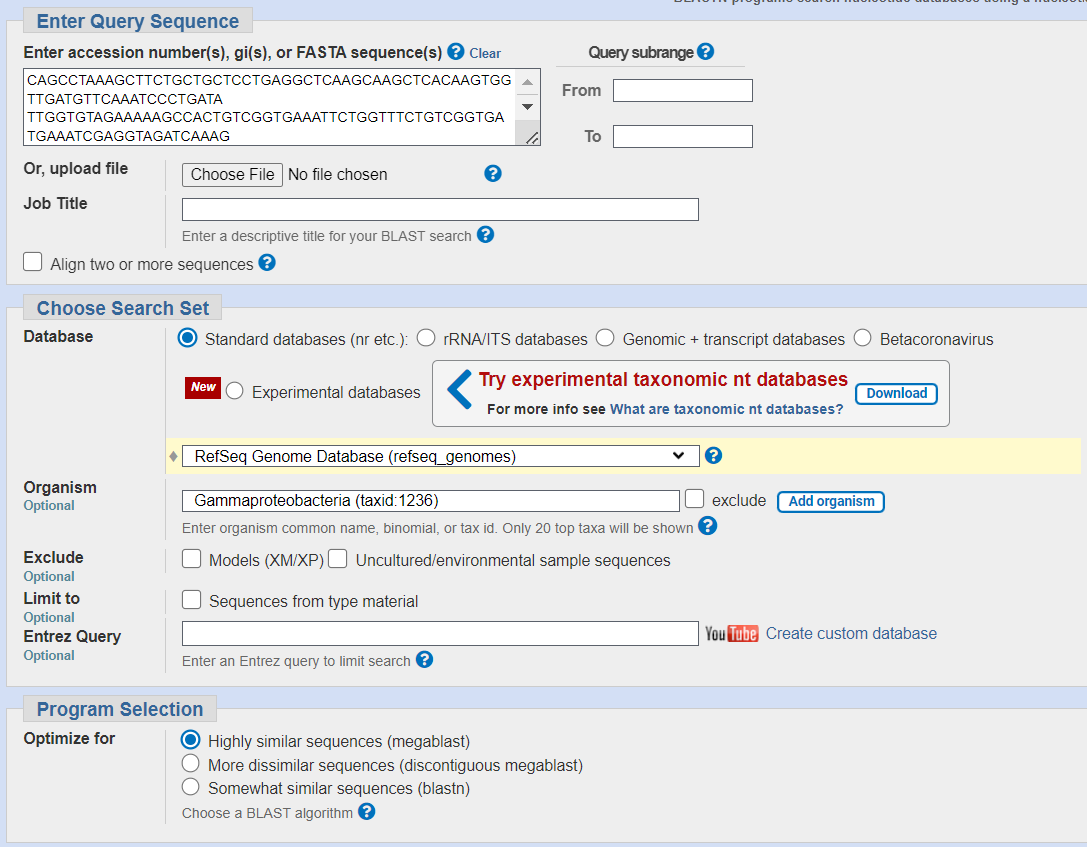
\includegraphics[width=0.9\textwidth]{blast_set}}
	
	(As specified in assignment)
	
	We got these alignments:
	
	\centerline{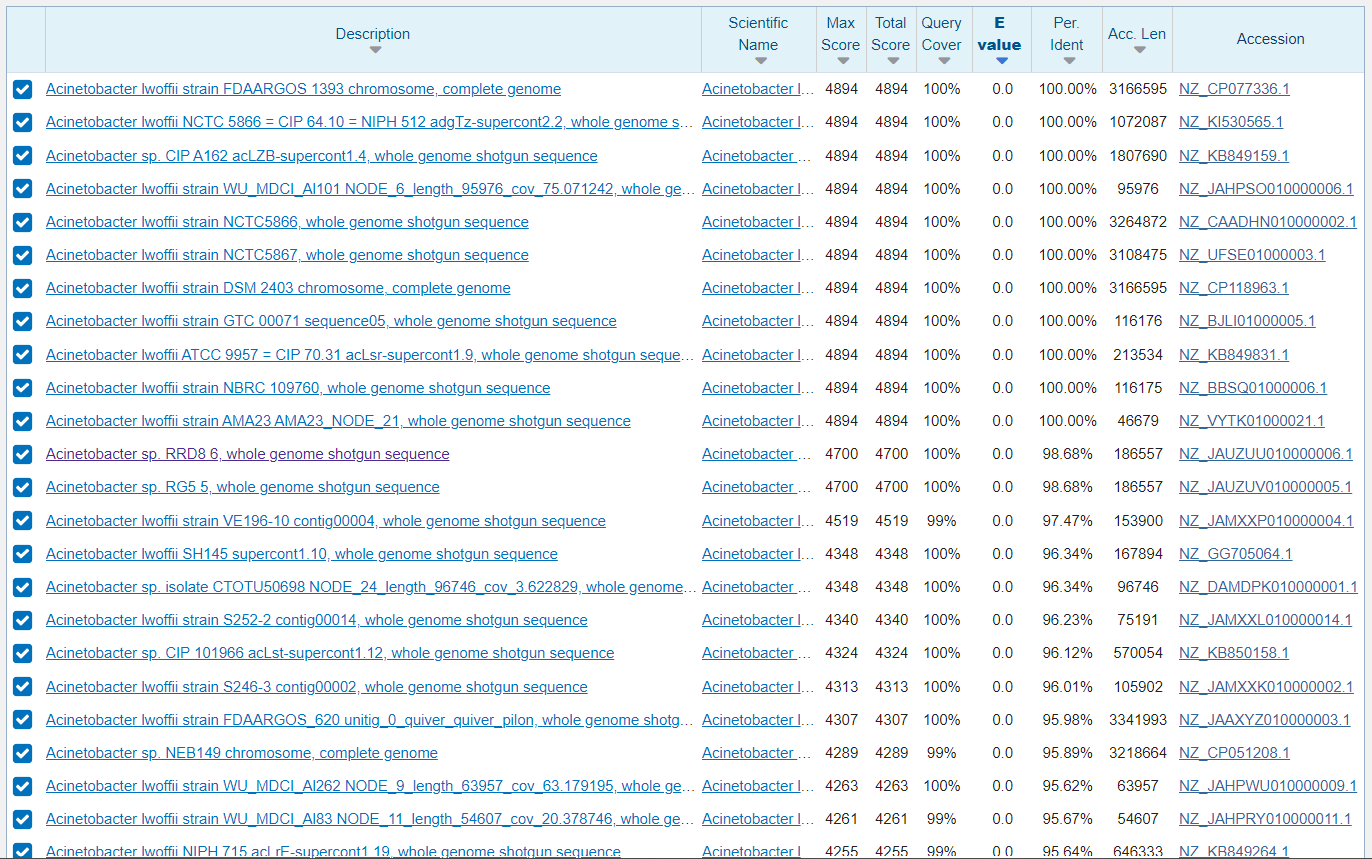
\includegraphics[width=1\textwidth]{blast_2}}
	
	We can see that in 11 sequences we got same highest score $4894$,  in all 11 cases algorithm identified $100\%$ of input sequence and E-value is approximately $0$.
	
	So most likely our sequence in part of genome of bacteria called Acinetobacter Iwofii.
	
	\subsection{}
	
	Now we will look at what kind od proteins might be encoded in our sequence, when we look for open reading frame with at least 180 codons we get 4 ORFs:
	
	\centerline{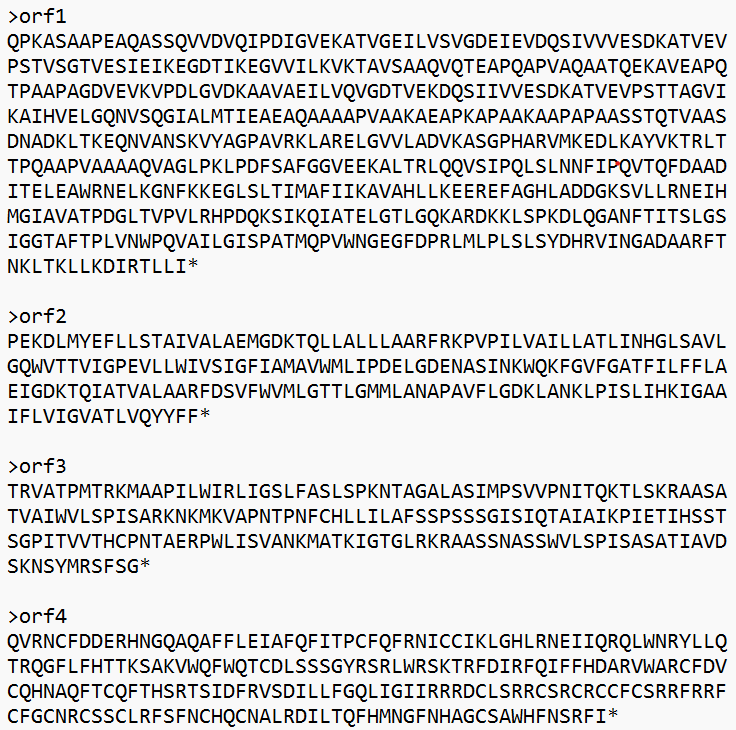
\includegraphics[width=0.8\textwidth]{orf0}}
	
	First two (ORF1 and ORF2) is on direct strand while last two (ORF3 and ORF4) are on reverse strand.
	
	\subsection{}
	
	Lastly we would like to see 3D structure of found proteins. We will look at ORF1 and ORF3. We used AlphaFold2 for this task.
	
	Now let's look firstly at ORF1:
	
	\centerline{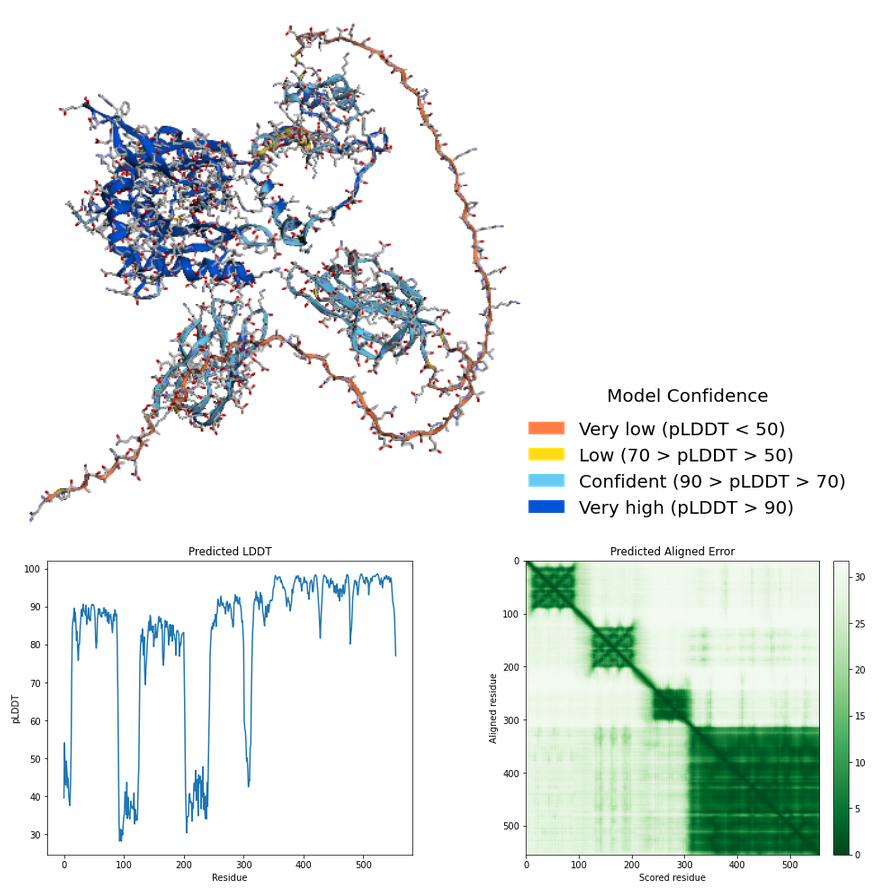
\includegraphics[width=1\textwidth]{orf1}}
	
	We can see that most of the structure (mostly complex parts) is colored blue which signifies pretty high accuracy, only parts with low confidence are structures connecting highly accurate complex structures. This is confirmed by "Predicted LDDT" plot where we can see most values are higher than 80 so highly accurate.
	
	On "Predicted aligned error" plot we can see 4 much darker squares which corresponds to 4 blue complex structure in 3D visualization. Dark cell mean that prediction error for relative positions of two those two amino acids (one from row and one from column) is low. So we can see that this protein seems to contain 4 domains.
	
	Now let's look at ORF3: 
	
	\centerline{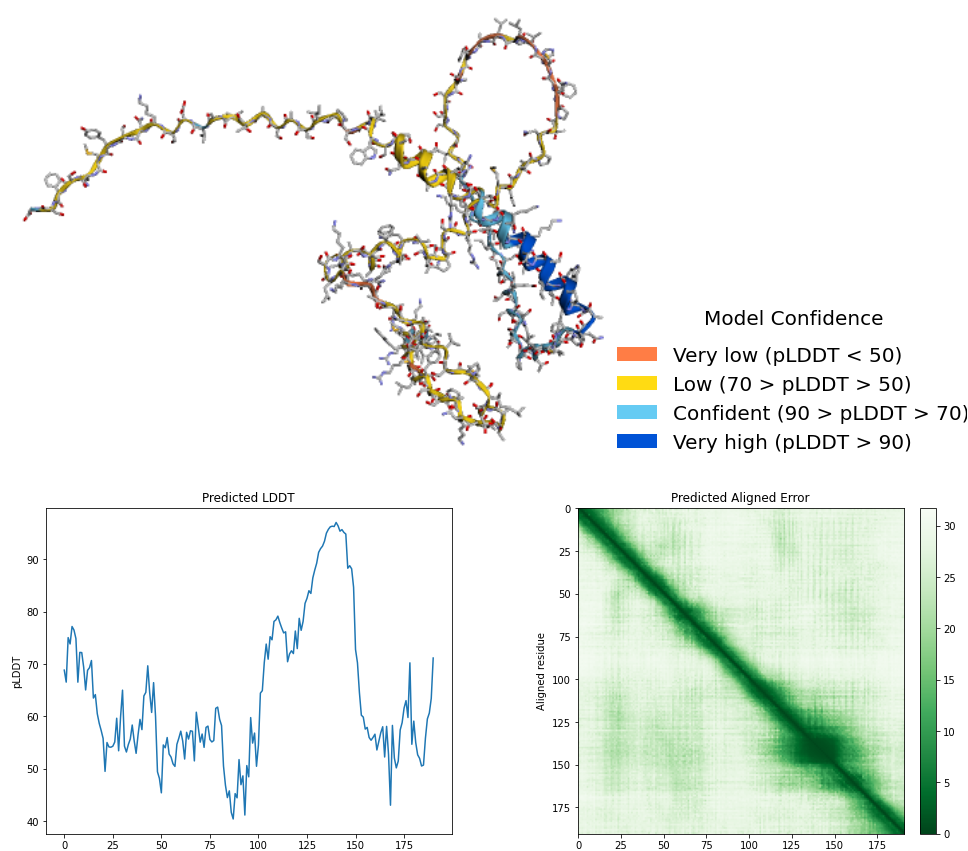
\includegraphics[width=1\textwidth]{orf3}}
	
	This time we don't see any highly complicated parts. Also we can see that most of structure is yellow which indicates low confidence, so AlphaFold is not sure if this is correct structure. "Predicted LDDT" confirms it as we can see that most values are lower than 50 with one notable spike which corresponds to small blue part in 3D visualization.
	
	"Predicted aligned error" plot also shows that other then amino acids right next to each other in sequence we have high error which means that relative position and/or orientation of almost any two amino acids is uncertain. One more information that we can get that algorithm was not able to find any notable domains.
	\\
	\\
	If we compare results for those two ORF we can say that prediction for ORF1 is much more reliable because we can be almost certain shape of most of a structure.
\end{document}